\documentclass{article}


\usepackage{amsmath} % math stuff
\usepackage{amssymb} % math stuff
\usepackage{array} % equations and stuff
\usepackage{bm} % bold math
%\usepackage{caption} % suppressed table numbering; incompatible with revtex, and longtable, I think
\usepackage{comment} % comment environment
%\usepackage{enumitem} % customization of enumeration, itemize, and description
\usepackage[T1]{fontenc} % font encoding for special characters, must also use scalable font package
\usepackage[margin=0.8in]{geometry} % paper sizes and margins (but be careful not to mess up pre-defined pages)
\usepackage{graphicx} % for graphics
%\usepackage{helvet} % default font is the helvetica postscript font
\usepackage{lipsum} % lorem ipsum filler text
\usepackage{lmodern} % scalable font?
\usepackage{longtable} % multi-page tables
\usepackage{mathrsfs} % math script font
\usepackage{mhchem} % easier chemical formula
\usepackage{microtype} % allows disabling of ligatures
%\usepackage{newcent} % new century schoolbook font
\usepackage{nicefrac}
\usepackage{parskip} % removes paragraph indentation, and adjusts paragraph skip, as well as list items
%\usepackage{setspace} % adjust text spacing and indents
\usepackage{siunitx} % decimal alignment
\usepackage{subfigure} % divided figures
%\usepackage{tabu} % extra table options
\usepackage{textcomp} % symbols
\usepackage{threeparttablex} % better footnotes with longtable
\usepackage{titling} % title placement
\usepackage{ulem} % strikethrough text
%\usepackage{url} % superceded by hyperref
\usepackage{verbatim} % verbatim environment
\usepackage{xcolor} % colors and color boxes
\usepackage{xspace} % commands that don't eat up white space
\usepackage{hyperref} % links and page setup; should always come last

\hypersetup{
	bookmarks=true,
	colorlinks=true,
	citecolor=blue,
	linkcolor=blue,
	urlcolor=blue,
	pdfstartview={XYZ null null 1.0} % default open view is 100%
}

\DisableLigatures[f]{encoding = *, family = * } % disable ff, fi, fl ligatures, without f option, it also disables -- = endash
\renewcommand{\arraystretch}{1} % extra vertical space in tables

\begin{document}

\pagestyle{empty} % don't number pages

% custom title
\begin{center}
{\LARGE Express Riddler}

\vspace{0.15in}

{\Large 24 April 2020}
\end{center}


\section*{Riddle:}

You and a friend are grilling two small square burger patties whose sides are 5 centimeters long.
However, you only have one slice of cheese remaining, which is also square and whose sides are 7 centimeters long.
You want to cut the slice so that all of the cheese is evenly split between the two patties, and no cheese is spilling over either patty and onto the grill.

What is the smallest number of cuts you need to make?
You can only make straight cuts, and you should assume that the cheese is stationary during the cutting process.

\section*{Solution:}

The answer is
\fcolorbox{red}{white}{\bf 2 cuts}\,.
I show the two cuts in the following diagram.

\begin{center}
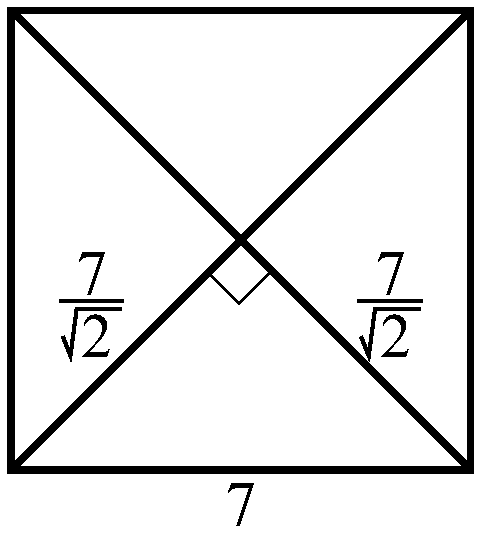
\includegraphics[width=2.5in]{cheese_slice.pdf}
\end{center}

With two cuts across the cheese's diagonals, there are now four 45-90-45 right triangles.
Each triangle has a hypotenuse of 7 and side lengths of $\nicefrac{7}{\sqrt{2}}\approx4.95$.
Two triangles can be put together at their hypotenuses, creating a square with side length just under 5, which fits inside a patty's area.

I must also prove that this result is in fact the minimum number of cuts, i.e., that there is no solution with one cut.
The longest cross section of the patties is the diagonal, which has length $5\sqrt{2}\approx7.07$, so any cheese portion must have a maximum cross section (at any angle) less than this.
The best single slice that minimizes both the total area and the maximum cross section is dividing two opposite sides in half, producing two identical rectangles.
This configuration leaves diagonals of the rectangles with length $\nicefrac{7\sqrt{5}}{2}\approx7.83$, which is too long.
Therefore, one cut is insufficient.

\end{document}